\documentclass{article}
% Uncomment the following line to allow the usage of graphics (.png, .jpg)
%\usepackage[pdftex]{graphicx}
% Comment the following line to NOT allow the usage of umlauts

\pagestyle{empty}
\usepackage[T2A]{fontenc}
\usepackage[utf8]{inputenc}
\usepackage[russian]{babel}
\usepackage{cmap}
\usepackage{amsthm}
\usepackage{amsmath}
\usepackage{units}
\usepackage{fancyhdr}
\usepackage{forloop}
\usepackage{amssymb}
\usepackage{url}
\usepackage{hyperref}
\usepackage{xcolor}
\usepackage[inline]{enumitem}

\usepackage{graphicx}
\usepackage{epstopdf}
\usepackage{caption}
\usepackage{subcaption}
\usepackage{amscd}


%\renewcommand{\thesection}{\arabic{section}.}

\renewcommand{\headrulewidth}{0.4pt}
\renewcommand{\footrulewidth}{0.4pt}

\fancyfoot[L]{стр. \thepage}
\fancyfoot[R]{\today}

\fancyhead[R]{Современные приложения ДА и ФА}
%For multipage documents only!
%\fancyfoot[L]{page: \thepage}
%Uncomment this for 1-page sheets
\fancyhead[L]{Перечислительная комбинаторика}
\fancyfoot[C]{}

\pagestyle{fancy}

\renewcommand{\baselinestretch}{1.0}
\renewcommand\normalsize{\sloppypar}

\setlength{\topmargin}{-0.5in}
\setlength{\textheight}{9.1in}
\setlength{\oddsidemargin}{-0.3in}
\setlength{\evensidemargin}{-0.3in}
\setlength{\textwidth}{7in}
\setlength{\parindent}{0ex}
\setlength{\parskip}{1ex}

\newcounter{problemset}
\newcounter{totalpages}
%Here you should set the total number of pages
\setcounter{totalpages}{1}

\def \topic {Семинар 2}

\def \Z {\mathbb Z}
\def \R {\mathbb R}
\def \P {\mathbb P}
\def \C {\mathbb C}
\def \vec {\boldsymbol}

\theoremstyle{definition}
\newtheorem{lemma}{Лемма}
\newtheorem{example}{Пример}
\newtheorem*{theorem}{Теорема}
\newtheorem*{definition}{Определение}

\usepackage{titlesec}

\makeatletter
\renewcommand{\section}{\@startsection
{section}%                   % the name
{1}%                         % the level
{\z@}%                       % the indent / 0mm
{-\baselineskip}%            % the before skip / -3.5ex \@plus -1ex \@minus 
%%-.2ex
{0.5\baselineskip}%          % the after skip / 2.3ex \@plus .2ex
{\centering\large\scshape}} % the style

\renewcommand{\subsection}{\@startsection
{subsection}%                % the name
{1}%                         % the level
{\z@}%                       % the indent / 0mm
{-\baselineskip}%            % the before skip / -3.5ex \@plus -1ex \@minus 
%%-.2ex
{0.5\baselineskip}%          % the after skip / 2.3ex \@plus .2ex
{\centering\large\scshape}} % the style
\makeatother

\begin{document}

\begin{center}

\newcommand{\HRule}{\rule{\linewidth}{0.5mm}}
\HRule \\[0.2cm]
{ \Large \bfseries \topic} %\\[0.2cm]
\HRule

\end{center}

\textsc{Ключевые слова: обыкновенные и экспоненциальные производящие функции, пентагональная теорема Эйлера, пилообразные перестановки, изоморфизм классов; модулярные формы, итерационные схемы}

\section{Производящие функции. Тизер номер 2.}

Здесь я хотел бы продолжить рекламу производящих функций и дать побольше 
мотивирующих примеров к их изучению. Весь первый раздел~--- это исключительно
реклама и обзор части существующих приложений. Мы не сможем во всей глубине
прочувствовать эти идеи прямо сейчас. Однако в конце документа можно встретить
тематические задачи по мотивам этих приложений.

\subsection{Эллиптические кривые и модулярные формы}
Этот пример я позаимствовал из книги Френкеля <<Любовь и Математика --- сердце
скрытой реальности>>, можно почитать английскую копипасту на просторах интернета
в блоге \cite{shimura-taniyama}. Ниже описаны результаты <<журналистского
расследования>>: я попытался дать элементарные, но точные формулировки
утверждений, которые я встретил в этой книге. Советую ознакомиться с задачами в
конце документа.

Пусть \( a_p \)~--- количество решений \( (x, y) \) кубического уравнения
\[
	y^2 + y = x^3 - x^2
\]
по модулю простого числа \( p \). Неважно откуда, слышал я такой факт\footnote{Оценка вида \( |a_p - p| < 2 \sqrt p \) встречается в \cite[Theorem 477]{number_theory}. Более точная оценка следует из гипотезы Бёрча -- Свиннертон-Дайера.}: количество решений \( a_p \) асимптотически приблизительно равно \( p \), то есть \( \lim_{p \to \infty} a_p / p = 1 \). Обозначим \( b_p = p - a_p \) разницу между асимптотическим и реальным числом решений, другими словами \textit{дефицит} числа решений. Например, по модулю \( 5 \) уравнение имеет \( 4 \) решения: \( (0,0 ), (0, 4), (1,0), (1,4) \), значит \( b_5 = 1 \).

% Weight 2 and level 11

Можно выписать псевдо-производящую функцию для последовательности чисел \( b_p
\). Я добавил приставку \textit{псевдо}, потому что в этой производящей функции нас
не будут интересовать коэффициенты при индексах, которые являются составными числами.
Таких производящих функций, естественно, существует бесконечно много, но среди
них есть одна особенно прекрасная.

Оказывается, псевдо-производящая функция для коэффициентов \( b_p \) может иметь вид
\[
	f(z) = z\prod_{n \geq 1}(1 - z^{n})^2(1 - z^{11 n})^{2} = 
	z(1 - z)^2(1 - z^{11})^{2}(1 - z^2)^2(1 - z^{22})^{2}(1 - z^3)^2(1 - 
	z^{33})^{2} \ldots
\]
Если раскрыть скобки, то получим
\[
	f(z) = z - 2z^2 - z^3 + 2z^4 + z^5 + 2z^6 - 2z^7 - 2z^9 - 2z^{10} + z^{11} 
	- 
	2z^{12} + 4z^{13} + \ldots
\]
Рассмотрим функцию \( f(z) \) как комплекснозначную функцию внутри комплексного
единичного круга \( {|z| < 1} \). При замене переменных (преобразование Фурье)
\( z = e^{2 \pi i \tau} \), переменная \( \tau \) пробегает значения \(
\mathrm{Im}\; \tau > 0 \).

\textbf{Внимание, опасный поворот!} Одному и тому же значению \( z \) сейчас
соответствует бесконечно много различных значений \( \tau \), потому что
комплексная экспонента \( 2 \pi i \)-периодична.

Рассмотрим группу \textit{дробно-линейных преобразований} \( \mathrm{PSL}(2,
\mathbb Z) \), то есть преобразований вида
\[
    \mathrm{PSL}(2, \mathbb Z) = \left\{
        \tau \to \dfrac{a \tau + b}{c \tau + d}, \quad
         ad - bc = 1, \, a, b, c, d \in \mathbb Z
    \right\} \enspace .
\]
Это преобразование переводит верхнюю полуплоскость \( \mathrm{Im}\; \tau \) в
верхнюю полуплоскость. Сложно сказать, как эта группа действует внутри
единичного круга, потому что теперь одной точке \( |z| < 1 \) может
соответствовать несколько точек вида \( \tau \), которые отличаются на нецелое
число.

Группа дробно-линейных преобразований \( \mathrm{PSL}(2, \mathbb
Z) \) имеет подгруппу \( \Gamma_0(N) \), определённую следующим образом:
\[
	\Gamma_0(N) = \left\{
		\tau \to \dfrac{a\tau + b}{c\tau + d} \colon ad - bc = 1, \, c \equiv 0
\bmod N
	\right\} \enspace .
\]

Выясняется следующий любопытный факт: группа \( \Gamma_0(11) \) является в
некотором смысле (сейчас скажу, в каком), группой симметрий указанной
производящией функции \( f(z) \). Говорят, что функция \( f(z) \) (после замены
переменных \( z = e^{2 \pi i \tau} \) является \textit{модулярной формой веса 2
для группы \( \Gamma_0(11) \)}, что в переводе на русский язык означает, что для
функции \( \varphi(\tau) = f(e^{2 \pi i \tau} ) \), \(f(z) = z \prod_{n \geq
1}(1 - z^n)^2 (1 - z^{11 n})^2 \) выполнено
\[
    \varphi\left(
        \dfrac{a\tau + b}{c \tau + d}
    \right)
     = (c \tau + d)^2 \varphi(\tau) \enspace .
\]
В общем случае, \textit{модулярной формой} веса \( k \) для группы \(
\Gamma_0(N) \) называется комплекснозначная функция \( f \colon \{\mathrm{Im}\;
z > 0\} \to \mathbb C \), для которой \(f (i \infty) = 0 \), и
\[
    f\left(
        \dfrac{az + b}{c z + d}
    \right)
     = (c z + d)^2 f(z) \quad \forall \begin{pmatrix}a & b \\ c&d
\end{pmatrix}  \in \Gamma_0(N) \enspace .
\]

Сухой итог изложенных здесь фактов: эллиптическая кривая \( y^2 + y = x^3 - x^2
\) называется \textit{модулярной}.

%\begin{theorem}
%	Проективные линейные преобразования переводят единичный круг в единичный круг. Пусть задана произвольная точка \( z_0 \) внутри едининого круга. Тогда существует проективно-линейное преобразование, которое переводит точку \( z_0 \) в центр круга.
%\end{theorem}

%Для того, чтобы визуализировать, как проективные преобразования действуют внутри круга, прилагаю картинку из википедии. Грубо говоря, с помощью таких преобразований можно любой жёлтый треугольничек перевести в любой другой треугольничек. См. рис \ref{fig:projective}. На рисунке может быть изображён график дискретнозначной функции, которая принимает 4 различных значения (чёрное, жёлтое, синее, красное).

%\begin{figure}[h]
%\centering
%\begin{subfigure}{.8\textwidth}
%	\centering
%	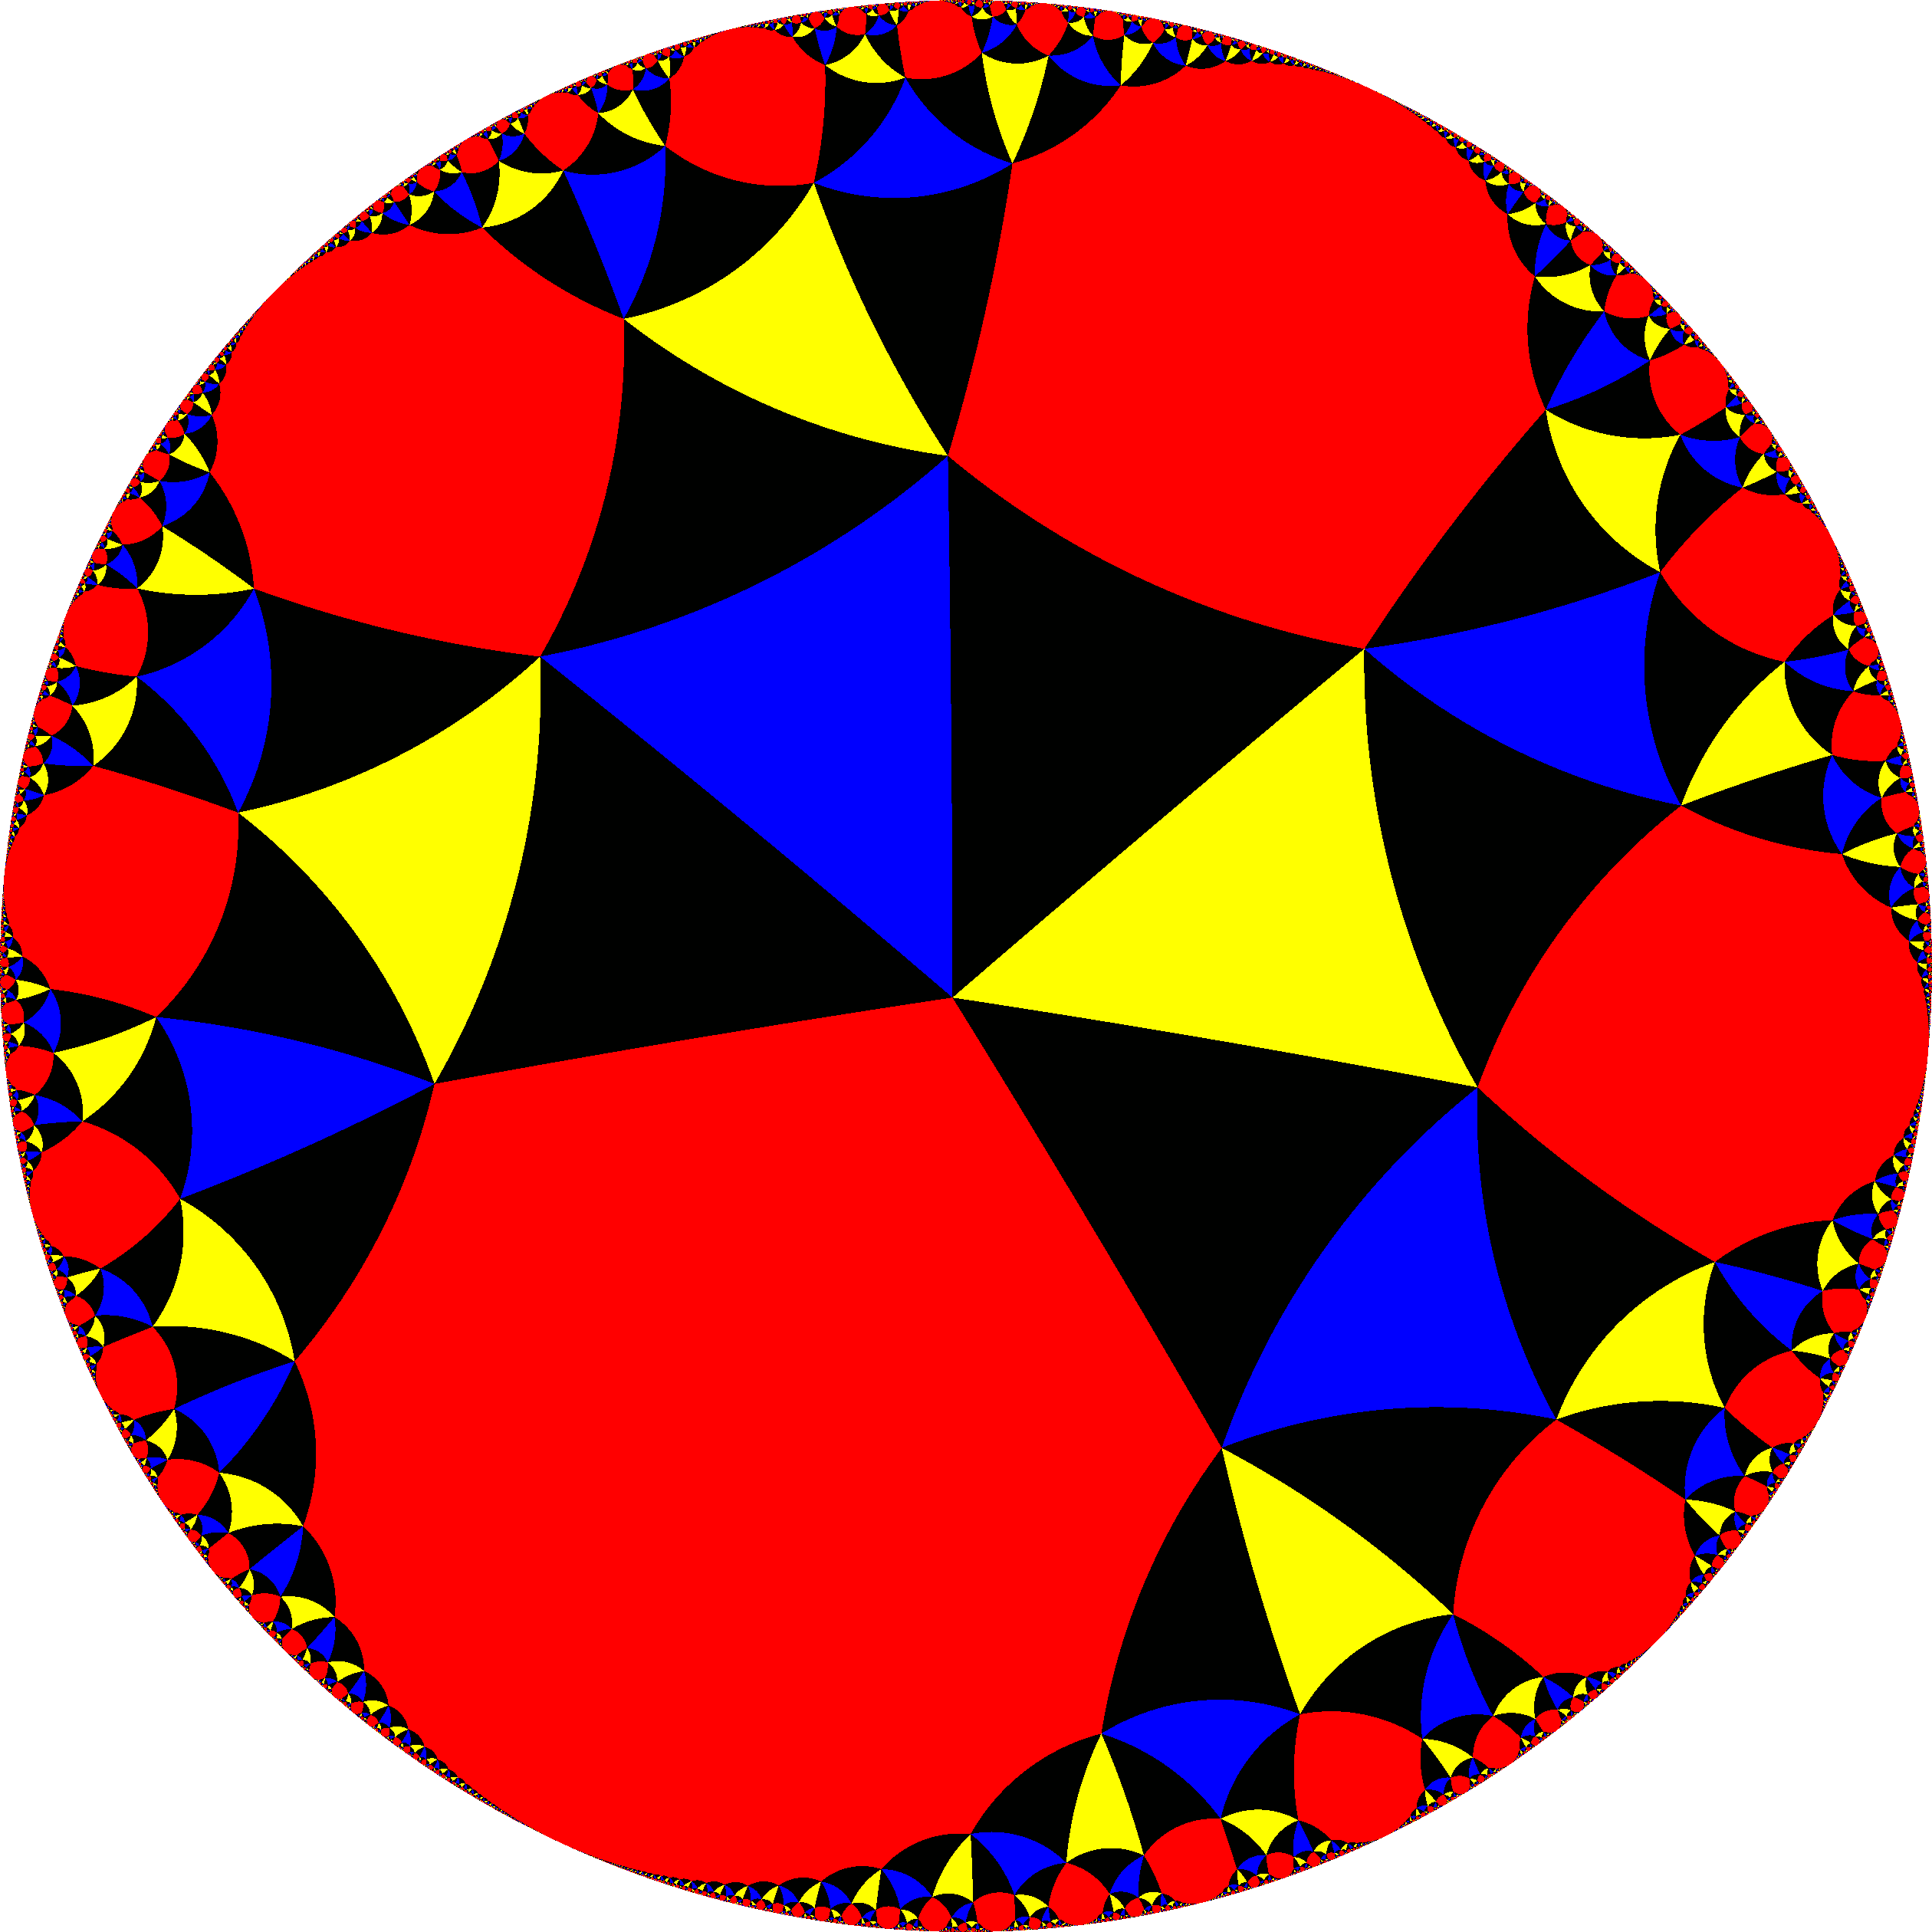
\includegraphics[width=.5\textwidth]{projective.png}
%\end{subfigure}%
%\caption{Замощение гиперболической плоскости.}
%\label{fig:projective}	
%\end{figure}

%Оказывается, группа \( \Gamma_0(11) \) является (проверьте!) группой симметрий для указанной выше функции \( f(z) \). Такие функции называются \textit{модулярными формами}. Про эллиптическую кривую, заданную уравнением \( {y^2 + y = x^3 - x^2} \) говорят, что она \textit{модулярна}.

\begin{theorem}[Гипотеза Симуры-Таниямы-Вейля]
Любая эллиптическая кривая модулярна.
\end{theorem}
Наверное, нет нужды напоминать, что это утверждение, также известное как \textit{теорема о модулярности}, (в более слабой формулировке) позволило математику Эндрю Уайлсу в 1994 году доказать Великую Теорему Ферма, а позже в 2001 году эту теорему доказали в общем случае другие математики. Обо всём этом можно прочитать и в википедии.

Теперь вы знаете, какая связь между такой теорией чисел и производящими функциями. Более подробную информацию об эллиптических кривых, решётках и модулярных формах, а также о мистической теореме Римана-Роха можно получить из многочисленных онлайн-курсов по этой теме в интернете, например здесь \cite{MF}.

\subsection{Метод Ньютона-Рафсона}
В методах оптимизации используется алгоритм \textit{Ньютона-Рафсона}, который 
ищет решение уравнения \( f(y) = 0 \), последовательно повторяя преобразования 
вида
\[
	\alpha^{\star} = \alpha - \dfrac{f(\alpha)}{f'(\alpha)} \enspace,
\]
стартуя с точки \( \alpha = 0 \). Если функция достаточно гладкая, то алгоритм 
сходится с квадратичной скоростью (под квадратичной скоростью понимается то, что с каждой итерацией удваивается число правильно найденных знаков после запятой). Применим алгоритм Ньютона-Рафсона к 
уравнению вида
\[
	y(z) = z \phi(y(z))
\]
для неизвестной функции \( y(z) \). Позже мы узнаем, что это уравнение 
соответствует различным типам деревьев. Например, для функции \( \phi(\tau) = 
e^{\tau} \) мы имеем помеченную конструкцию <<дерево это корневая вершина и 
множество поддеревьев>>. Применение алгоритма даёт последовательность 
производящих функций \(  y_{m}(z) \), таких, что
\[
	y_{m+1}(z) = y_{m}(z) + \dfrac{z \phi(y_{m}(z)) - y_{m}(z)}{1 - z 
	\phi'(y_m(z))}, \qquad y_0(z) = 0 \enspace .
\]
Можно показать (\cite[I.64, p.88]{ac}, \cite[Section 3.3]{species}), что у функций \( y_{m}(z) \) и \( y(z) 
\) совпадают первые \( 2^m - 1 \) коэффициентов.

\subsection{Нигде не сходящиеся функции}

Рассмотрим обыкновенную производящую функцию для числа перестановок
\[
	f(z) = \sum_{n \geq 0} n! z^n \enspace .
\]
Радиус сходимости функции \( f(z) \) равен нулю. Вообще, в комбинаторике, по 
всей видимости, гораздо <<больше>> объектов, чья производящая функция 
расходится. Для обыкновенных производящих функций коэффициенты сходящейся 
фунции должны расти не быстрее, чем \( C^{n} \), а для экспоненциальных 
производящих функций коэффициенты имеют вид \( \dfrac{a_n}{n!} \), и по формуле 
Стирлинга \( a_n \) должно расти не быстрее, чем \( C^{n \log n} \). Для 
сравнения, количество графов на \( n \) вершинах равно \( 2^{{n \choose 2}} \), 
и показатель экспоненты уже квадратичный. Число помеченных деревьев, согласно 
теореме Кэли, равно \( n^{n-1} \), что соответствует \( C^{n \log n} \), 
поэтому получается так, что экспоненциальная производящая функция \( \sum_{n > 
0} \dfrac{n^{n-1}}{n!} x^n \) аналитична в нуле.

Но примечательно то, что функция \( f(z) \) удовлетворяет дифференциальному 
уравнению
\[
	z^2 f'(z) + (z-1) f(z) = 0 \enspace ,
\]
и это уравнение имеет комбинаторный смысл. Среди методов аналитической 
комбинаторики есть и такие, которые позволяют из соответствующих 
дифференциальных уравнений находить асимптотику коэффициентов, даже если 
функция не аналитична в нуле.

\subsection{Эволюция случайных графов}

Модель случайного графа Эрдёша-Реньи известна многим, потому что она довольно 
простая, и пользуются ей не только люди, занимающиеся комбинаторикой, а также 
вероятностники, статистики, и вообще много разных Computer-Scientist-ов. 
Модель \( G(n,p) \) это случайный граф, построенный на \( n \) вершинах, где 
каждое ребро появляется независимо от других с вероятностью \( p \in [0, 1] \).
Оказывается, Эрдёш и Реньи изначально рассматривали не \( G(n,p) \) модель с 
независимыми 
рёбрами, а модель \( G(n,m) \), в которой граф выбирается случайно 
равновероятно среди множества графов с \( n \) вершинами и \( m \) рёбрами. В 
общем-то для \( n \to \infty \), \( m \to \infty \) эти модели становятся 
асимптотически эквивалентными, и, насколько мне известно, все свойства, 
доказанные для одной модели, выполняются и для другой, в предположении, что 
среднее количество рёбер совпадает.
Аппарат аналитической комбинаторики и производящих функций даёт очень 
эффективный метод для получения свойств графов в модели \( G(n,m) \).
\begin{enumerate}
\item[\( \bullet \)] Если число рёбер \( m  = c n \), \( c < 1/2 \), то размер 
наибольшей компоненты связности имеет порядок \( \Theta(\log n) \)
\item[\( \bullet \)] Если число рёбер \( m  = c n \), \( c = 1/2 \), то размер 
наибольшей компоненты связности имеет порядок \( \Theta(n^{2/3}) \)
\item[\( \bullet \)] Если число рёбер \( m  = c n \), \( c > 1/2 \), то размер 
наибольшей компоненты связности имеет порядок \( \Theta(n) \).
\end{enumerate}
Можно исследовать не только размер компоненты связности, а многие другие 
свойства, как вероятность графа быть планарным, вероятность содержать ровно 
одну <<гигантскую>> компоненту при последовательном добавлении рёбер, и так 
далее. Она, кстати, равна \( 5\pi / 18 \), эта вероятность. Подробнее см. 
\cite{giant_component}.

Лично мой вклад в этой область, полученный на двухмесячной стажировке в 
Париже (в соавторстве с научным руководителем Vlady Ravelomanana), заключался в 
том, что мы исследовали множество графов \( G(n,m,\Omega) 
\), где граф выбирается случайно равновероятно среди множества графов с \( n \) 
вершинами и \( m \) рёбрами с дополнительным ограничением: степень каждой 
вершины должна лежать в заданном множестве \( \Omega = \{\omega_1, \omega_2, 
\ldots \} 
\), конечном или бесконечном. Основной результат заключался в том, что 
критическая точка \( 1/2 \) (см. выше) может переместиться влево или вправо в 
пределах отрезка \( [0, 1] \) в зависимости от выбора множества \( \Delta \). 
Значение критической точки определяется неким  \textit{характеристическим 
уравнением} для экспоненциальной производящей функции множества \( \Omega \).

\subsection{Производящие функции от нескольких аргументов}

Пусть нас интересует ответ на вопрос <<сколько существует деревьев на \( n \) 
помеченных вершинах, имеющих высоту \( k \)>>? Здесь участвуют два параметра и 
нужно рассматривать производящую функцию от двух переменных, экспоненциальную 
по \( x \) и обыкновенную по \( y \):
\[
	F(x, y) = \sum_{n \geq 0} \sum_{k \geq 0} \dfrac{c_{n,k}}{n!} x^n y^k 
	\enspace ,
\]
где \( c_{n,k} \)~--- количество деревьев. Оказывается, что это не просто 
обозначение, а между производящими функциями от одной и от нескольких 
переменных существует тесная взаимосвязь, и можно естественным образом 
переходить к новым конструкциям, добавляя \textit{параметры}, о которых мы 
хотим знать. Каждому параметру соответствует своя переменная.

Ясно, что такие задачи решать сложнее, чем просто узнавать число деревьев. 
Многие техники, разработанные для \textit{одной переменной}, в частности 
\textit{метод анализа седловой точки ТФКП}, обобщается на несколько переменных 
в книге Analytic Combinatorics in Several Variables \cite{acsv}. Там можно 
найти и методы алгебраической топологии, и 
теорию Морса, и базисы Грёбнера~--- в общем все эти интересные слова, в которых 
я пока ничего не понимаю, но наверное когда-нибудь пойму~--- обязательно вам 
расскажу.

\section{В предыдущих сериях}

Кратко резюмирую, о чём мы должны сейчас иметь представление, чтобы двигаться 
дальше.
\begin{enumerate}
	\item Объект это пара \( (U, \gamma) \), где \( \gamma \) задаёт некоторую 
	структуру на \( U \), а множество \( U \)~--- множество атомов~--- 
	представляет из себя множество вида \( \{ 1,2,\ldots, n \} \) для 
	некоторого \( n \). Объекты объединяются в \textit{классы}.
	
	Перестановки объектов \( \sigma \colon U \to U \) действуют на структурах. 
	Действие перестановки на структуре обозначается \( \sigma \gamma \).
	\item Два объекта из одного класса \( a, b \) \textit{идентичны} (или 
	совпадают как помеченные структуры), если их структуры \( \gamma_a,	
	\gamma_b \) тоже совпадают. Два объекта из одного класса \( a, b \) 
	\textit{изоморфны} (или совпадают как непомеченные структуры), если 
	существует перестановка \( \sigma \) такая, что \( \sigma \gamma_a = 
	\gamma_b \).
	\item Классу объектов \( \mathcal A \) можно сопоставить как 
	\textit{обыкновенную производящую функцию}
	\[
		\widetilde A(x) = \sum_{n \geq 0} a_n x^n \enspace ,
	\]
	где \( a_n \)~--- количество различных \textit{неизоморфных} объектов, так 
	и \textit{экспоненциальную производящую функцию}
	\[
		A(x) = \sum_{n \geq 0} \dfrac{b_n}{n!} x^n \enspace ,
	\]
	где \( b_n \)~--- количество различных \textit{неидентичных} объектов.
	\item На классах объектов определены различные операции: для двух классов 
	\( \mathcal A, \mathcal B \) определены \( \mathcal A \sqcup \mathcal B \), 
	\( \mathcal A \times B \), для одного класса: \textsc{seq}\( 
	(\mathcal A) \).
	\item Хороший вопрос на понимание: почему для непомеченных классов есть две 
	операции: множество и мультимножество \textsc{pset}, \textsc{mset}, а для 
	помеченных только \textsc{set}? Можно ли определить эти операции для 
	комбинаторных классов, не думая про способ пометки объектов?
	\item\( ^{\ast} \) \footnotesize Чтобы наконец избавиться от недоразумения 
	в вопросе <<что такое структура \( \gamma \)>> и окончательно поставить 
	точку в этом вопросе, можно дать следующее формальное
	определение \cite[Definition 3, page 5]{species}. 
	\begin{definition}
	 	\textit{Классом объектов} \( \mathcal A \) называется \textit{правило} 
	 	\( F \), которое
	 	\begin{enumerate}
		 	\item Каждому конечному множеству \( U \) вида \( \{ 1, 2, \ldots, 
		 	n \} \) сопоставляет конечное множество \( F[U] \). (В старых 
		 	терминах это множество объектов заданного размера \( n \)).
		 	\item Каждой биекции \( \sigma \colon U \to V \) сопоставляет 
		 	функцию \( F[\sigma] \colon F[U] \to F[V] \). (Эта функция 
		 	осуществляет естественный транспорт между структурами)
		 	
		 	Функция \( F[\sigma] \) должна удовлетворять следующим 
		 	\textit{функториальным} свойствам:
		 	\begin{enumerate}
			 	\item Для любых биекций \( \sigma \colon U \to V \), \( \tau 
			 	\colon V \to W \),
			 	\[
			 		F[\tau \circ \sigma] = F[\tau] \circ F[\sigma] \enspace ,
			 	\]
			 	\item Для тождественного отображения \( \mathrm{Id}_{U} \colon 
			 	U \to U 
			 	\),
			 	\[
			 		F[\mathrm{Id}_{U}] = \mathrm{Id}_{F[U]} \enspace .
			 	\]
		 	\end{enumerate}
	 	\end{enumerate}
	\end{definition}
	Это определение сосредотачивается не на теоретико-множественной или 
	комбинаторной внутренней природе структуры объектов, а на 
	\textit{функториальном подходе}, который рассматривает поведение объектов 
	при действии перестановок.
\end{enumerate}

\section{Интересные примеры}

Часто встречаются примеры с бесконечным произведением. Бесконечное произведение 
корректно определено, если при раскрытии скобок каждый коэффициент при \( x^n 
\) оказывается конечным числом.

Один из таких примеров был в мотивирующей части этого семинара. Чтобы не 
спойлерить решения задач, рассмотрим достаточно известный пример, известный как 
\textbf{пентагональная 
теорема Эйлера}. Обычно эта теорема является частью изложения более сложной 
теории, связанной с эллиптическими тета-функциями, тождеством Якоби как 
обобщениями теоремы Эйлера, а также q-функциями для разбиений чисел. Мы в эти 
дебри пока не будем лезть, но я оставлю ссылку на соответствующий раздел в 
книге Стенли \cite[Section 1.8]{stanley1}.

\begin{theorem}[Пентагональная теорема Эйлера]
	Пусть \( f(z) = \prod_{n \geq 1}(1 - x^n) \). Тогда при раскрытии скобок 
	функция \( f(z) \) имеет вид
	\[
		f(z) = 1 - x - x^2 + x^5 + x^7 - x^{12} - x^{15} + x^{22} + x^{26} - 
		\ldots
	\]
	Все коэффициенты после раскрытия скобок равны \( 0, +1, -1 \), знаки 
	коэффициентов чередуются по принципу два минуса, два плюса. Показатели 
	степеней это так называемые \textit{пентагональные числа}. В общем случае,
	\[
		f(z) = \sum_{q = -\infty}^{+\infty} (-1)^{q} x^{(3q^2+q)/2} \enspace .
	\]
\end{theorem}

\begin{proof}
\begin{figure}[h]
\centering
\begin{subfigure}{.8\textwidth}
	\centering
	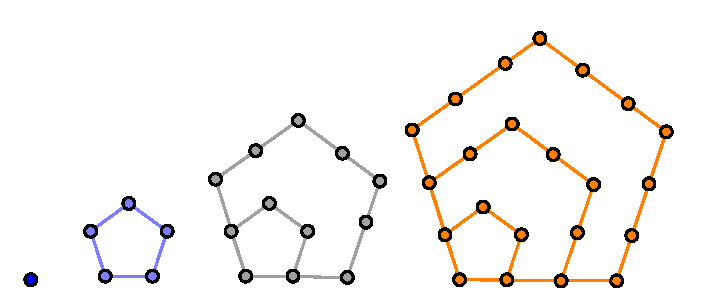
\includegraphics[width=.7\textwidth]{pentagonal}
\end{subfigure}%
\caption{Пентагональные числа 1, 5, 12, 22}
\label{fig:pentagonal}	
\end{figure}
	При раскрытии скобок коэффициент при \( x^n \) равен сумме чисел вида \( 
	-1, +1 \) где каждое слагаемое соответствует разбиению числа \( n \) на 
	различные слагаемые, а знак определяется чётностью числа слагаемых в 
	разбиении. Значит, нужно построить взаимно однозначное соответствие между 
	разбиениями с чётным и нечётным числом слагаемых.
	
	Предъявим комбинаторное биективное доказательство, следуя изложению 
	\cite[Proposition 1.8.7]{stanley1}. Читатель может подумать над 
	альтернативными способами построить биекции для числа разбиений на чётное и 
	нечётное число различных слагаемых.
	
	Пусть имеется разбиение \( \lambda \) числа \( n \) на множество различных 
	слагаемых. 
	Слагаемые можно упорядочить по убыванию, затем составить 
	\textit{диаграмму}, в которой каждому слагаемому \( s_i \) соответствует 
	строка, состоящая из \( s_i \) точек. На рисунке \ref{fig:ferrer_1} 
	изображена диаграмма (Феррера) для разбиения \( 23 = 7+6+5+3+2 \). 
	Обозначим нижнюю строку этой диаграммы \( L_{\lambda} \), а самую правую 
	<<диагональ>> \( D_{\lambda} \). Возможны два случая: \( L_{\lambda} > 
	D_{\lambda} \) или \( L_{\lambda} \leq D_{\lambda} \).
	\begin{enumerate}
	\item Случай \( L_{\lambda} \leq D_{\lambda} \). Преобразование состоит в 
	том, чтобы удалить \( L_{\lambda} \) и поместить его параллельно \( 
	D_{\lambda} \), чтобы оборазовать следующую диагональ.
	\item Случай \( L_{\lambda} < D_{\lambda} \). Необходимо совершить обратное 
	преобразование: удалить \( D_{\lambda} \) и поместить его под \( 
	L_{\lambda} \).
	\end{enumerate}
\begin{figure}[h]
\centering
\begin{subfigure}{.33\textwidth}
	\centering
	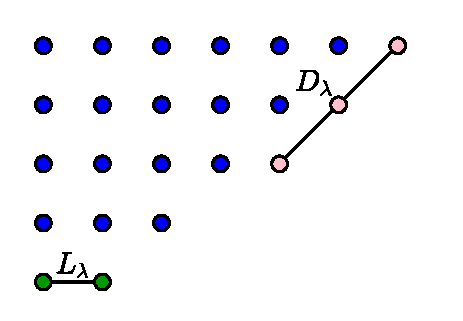
\includegraphics[width=.8\textwidth]{ferrer_1}
	\caption{Случайное разбиение}
	\label{fig:ferrer_1}	
\end{subfigure}%
\begin{subfigure}{.33\textwidth}
	\centering
	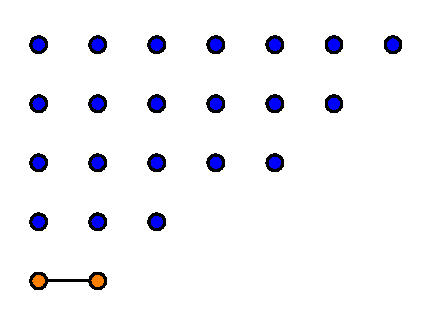
\includegraphics[width=.7\textwidth]{ferrer_2}
	\caption{Исходная диаграмма}
	\label{fig:ferrer_2}	
\end{subfigure}
\begin{subfigure}{.33\textwidth}
	\centering
	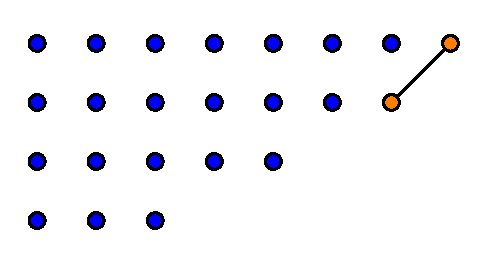
\includegraphics[width=.8\textwidth]{ferrer_3}
	\caption{После преобразования}
	\label{fig:ferrer_3}	
\end{subfigure}
\caption{Диаграммы Феррера для разбиений}
\end{figure}
Ясно, что преобразование является инволюцией (то есть двухкратное 
повторение возвращает нас к исходной диаграмме), и оно меняет чётность 
числа слагаемых. Однако, возникают ситуации, когда преобразованная 
диаграмма не является корректной диаграммой Феррера. Возможны ровно два случая: 
\( \lambda = (2k-1, 2k-2, \ldots,k) \) и \( \lambda = (2k, 2k-1, \ldots, k+1) 
\), см. рисунок \ref{fig:ferrer_4}. Этим случаям соответствуют \( n = k(3k-1)/2 
\) и \( n = k(3k+1)/2 \) соответственно.
\begin{figure}[h]
\centering
\begin{subfigure}{.4\textwidth}
	\centering
	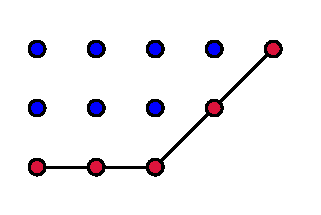
\includegraphics[width=.5\textwidth]{ferrer_4}
%	\caption{Случайное разбиение}
%	\label{fig:ferrer_1}	
\end{subfigure}%
\begin{subfigure}{.4\textwidth}
	\centering
	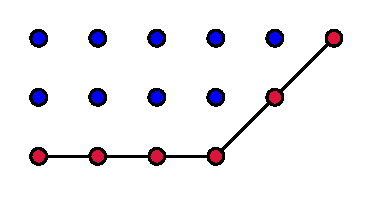
\includegraphics[width=.6\textwidth]{ferrer_5}
%	\caption{Исходная диаграмма}
%	\label{fig:ferrer_2}	
\end{subfigure}
\caption{<<Плохие разбиения>>}
\label{fig:ferrer_4}	
\end{figure}
\end{proof}
Числа вида \( k(3k-1)/2 \) называются \textit{пентагональными числами}, см. 
рисунок \ref{fig:pentagonal}.

Теперь, когда мы научились раскрывать скобки в бесконечном произведении, решим 
несложную задачку на применение экспоненциальных производящих функций, просто 
чтобы прокачать наше чувственное восприятие этих структур.

\begin{example}[{\cite[Пример 3.2.13, стр. 167]{gouldenjackson}}]
	Найти количество последовательностей длины \( \ell \) над \( \{ 0,1,2 \} 
	\), в которых никакой символ не встречается точно \( p \) раз.
	
	Оказывается, строки можно рассматривать как помеченные объекты, и как 
	непомеченные объекты. Пусть строка имеет вид
	\[
		s = \sigma_1 \sigma_2 \ldots \sigma_\ell  \enspace ,
	\]
	Меткой символа \( \sigma_i \) является \( i \). Покажем, что производящая 
	функция помеченных конфигураций имеет вид
	\[
		S(x) = \left(
			e^{x} - \dfrac{x^p}{p!}
		\right)^{3} \enspace .
	\]
	Так как каждый символ равен \( 0, 1, 2 \), то строка задаёт разбиение 
	помеченных объектов в <<ящики>> с номерами \( 0, 1, 2 \). Так как никакой 
	символ не встречается ровно \( p \) раз, то запрещены <<ящики>>, содержащие 
	ровно \( p \) объектов. Таким образом, раскрывая скобки, получаем 
	количество таких последовательностей:
	\[
		\ell! [x^\ell] \left(
					e^{x} - \dfrac{x^p}{p!}
				\right)^{3} = 3^{\ell} - 3 {\ell \choose p} 2^{\ell - p} + 3 
				{2p \choose p}{\ell \choose 2p} - \dfrac{\ell!}{p!^3} 
				\delta_{3p, \ell} \enspace .
	\]
	Здесь \( \delta_{x,y} = 1 \), если \( x = y \), и \( \delta_{x,y} = 0 \), 
	если \( x \neq y \)~--- дельта-символ Кронекера.
\end{example}

Далее, в лучших традициях фолк-семинара, я разберу ещё один известный пример, 
который был анонсирован в самом начале первого семинара~--- число пилообразных 
перестановок. Теории приходят и уходят, а примеры остаются\footnote{Хотя другой 
афоризм гласит, что лучшая практика --- это хорошая теория. Впрочем, никакого 
противоречия я здесь не вижу.}. Однако после того, как мы разберём этот пример, 
я рискну здесь изложить элементы theory of species, чтобы 
придать некую завершённость происходящему.

\begin{example}
Производящая функция пилообразных down-up перестановок с нечётным числом вершин 
равна \( \tan x \). Под пилообразной down-up перестановкой понимается 
последовательность \( (a_1, a_2, \ldots, a_n) \), составленная различных чисел 
\( \{ 1, 2, \ldots, n \} \), где \( a_1 < a_2 \), \( a_2 > a_3 \), \( \ldots 
\), \( a_{n-1} > a_n \).

\begin{figure}[h]
\centering
	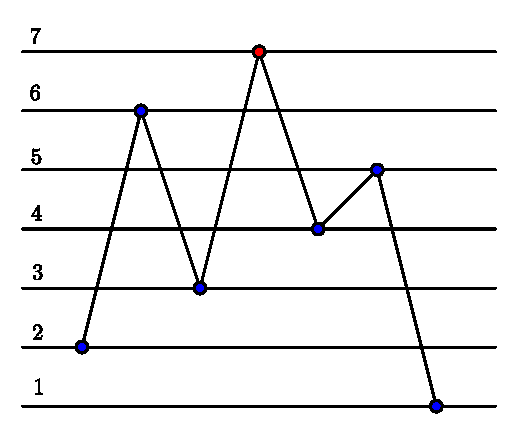
\includegraphics[width=.42\textwidth]{saw_permutation}
\caption{Максимальный элемент пилообразной перестановки}
\label{fig:saw_permutations}	
\end{figure}
	
Как часто бывает, чтобы понять, что из себя представляют пилообразные 
перестановки, нужно ввести на них некую <<алгебру>>. Давайте запишем ЭПФ 
пилообразных перестановок и продифференцируем её.
\[
	f(x) = \sum_{n \geq 0} \dfrac{a_n}{n!} x^n \enspace ,
	f'(x) = \sum_{n \geq 1} \dfrac{a_n}{(n-1)!} x^{n-1} = \sum_{n \geq 0} 
	\dfrac{a_{n+1}}{n!}x^{n}\enspace .
\]
Производящая функция \( f'(x) \) описывает класс, в котором объекты размера \( 
n \)~--- это объекты размера \( n+1 \) исходного класса с дополнительной 
\textit{стирающей маркировкой} атома с номером \( n+1 \). 

Заметим, что максимальный атом пилообразной down-up перестановки обязательно 
стоит на нечётной позиции, потому что на чётных позициях находятся локальные 
минимумы. Подпоследовательности, стоящие слева и справа от маркированного 
атома, имеют обе нечётную длину, и обе являются пилообразными. Читателю 
предоставляется проверить, что выполнено следующее соотношение:
\[
	\dfrac{df(x)}{dx} = f^2(x) + 1 \enspace .
\]
\end{example}
Это дифференциальное уравнение с начальным условием \( f(0) = 0 \) решается 
методом разделения переменных:
\[
	\dfrac{df}{f^2 + 1} = dx, \quad
	\int \dfrac{df}{f^2 + 1} = \int dx, \quad
	\arctan f(x) = x, \quad
	f(x) = \tan x \enspace .
\]

\section{Изоморфизм классов и почему это может быть важно}

Мы уже знаем, что экспоненциальная производящая функция \textit{перестановок} 
имеет вид
\[
	f(z) = \dfrac{1}{1 - z} \enspace .
\]
Эта производящая функция совпадает с ЭПФ \textit{последовательности атомов}, и 
не зря: любую перестановку \( n \) элементов можно задать с помощью 
последовательности различных чисел от \( 1 \) до \( n \). Тем не менее, я 
сейчас покажу, что \textit{последовательности} и \textit{перестановки} это два 
различных (неизоморфных) класса объектов, у которых совпадают экспоненциальные 
производящие функции (но не совпадают обыкновенные производящие функции).

Действительно, перестановка, по определению, это биективное отображение 
множества \( \{ 1, 2, \ldots, n \} \) в множество \( \{ 1, 2, \ldots, n \} \). 
Графически здесь достаточно представлять, что тип перестановки задаётся её 
\textit{цикловым разложением}. Две перестановки, согласно нашему определению, 
называются \textit{изоморфными}, если существует третья перестановка \( \sigma 
\), такая, что действие перестановки на первом объекте переводит его во второй 
объект. Внимательный читатель заметит, что это действие является в точности 
действием сопряжениями~--- следовательно, две перестановки изоморфны, если их 
цикловое разложение одинаковое.

Теперь мы знаем, что количество неизоморфных перестановок на \( n \) элементах 
это количество способов представить \( n \) в виде суммы мультимножества 
натуральных чисел. Это позволяет нам выписать обыкновенную производящую функцию:
\[
	\widetilde{F}(z) = \dfrac{1}{(1-z)(1-z^2)(1-z^3) \ldots} \enspace .
\]
Я был удивлён не меньше вашего. Всё сказанное заставляет переосмыслить пример с 
пилообразными перестановками.

\section{Задачи}

\begin{enumerate}
\item(10 очков) Докажите формулу для производящей функции числа решений уравнения \( y^2 + y = x^3 - x^2 \).

\item(3 очка) Докажите, что функция Эйзенштейна
\[
	G_k(\tau) = \sum_{m,n\in \mathbb Z, \, (m,n) \neq (0,0)} \dfrac{1}{(m \tau + n)^k}
\]
удовлетворяет функциональному уравнению
\[
	G_k\left( \dfrac{a \tau + b}{c \tau + d}\right) = (c \tau + d)^2 G_k(\tau), \qquad \forall a,b,c,d \in \mathbb Z, \, ad - bc = 1 \enspace ,
\]
то есть функция Эйзенштейна является модулярной формой веса 2.

\item(7 очков) Докажите, что эллиптическая кривая \( y^2 + y = x^3 - x^2 \)
является модулярной веса \( 2 \) для группы \( \Gamma_0(11) \), то есть для указанной производящей функции \( f(z) \) (см. раздел 1.1) после переобозначения переменных \( \varphi(\tau) = f(e^{2 \pi i \tau}) \), мы имеем
\[
	\varphi \left(\dfrac{a \tau + b}{c \tau + d}\right) = (c \tau + d)^{2} \varphi (\tau), \quad
	(a,b,c,d) \in \Gamma_0(11) \enspace .
\]
Многочисленные подсказки к решению этой задачи можно найти в
\cite[Proposition 3.2.2]{first_course_modular_forms}. Оказывается, нужно
воспользоваться тем фактом, что функция \( \varphi(\tau) \) представляется в
виде \( \eta(\tau)^k \eta(N \tau)^k  \), где \( N = 11, \, k = 2 \), \( k(N+1) =
24 \), и функция \( \eta(\tau) = \tau^{\frac{1}{24}} \prod_{n \geq 1}(1 -
\tau^n) \)~--- функция Дедекинда.

\item(3 очка) Пусть задан формальный степенной ряд \( f(t) = \sum_{n \geq 1} c_n t^n \), \( f'(0) \neq 0 \), а также неизвестная функция \( t(x) \), удовлетворяющая условию
\[
	f(t(x)) = x \enspace .
\]
Обозначим \( R(t) = t / f(t) \).
Рассмотрим итерационную схему для нахождения неизвестного формального степенного ряда \( t(x) \):
\[
	t^{(0)}(x) = 0, \quad
	t^{(i+1)}(x) = t^{(i)}(x) + \dfrac{x R(t^{(i)}) - t^{(i)}}{1 - x R'(t^{(i)})} \enspace .
\]
Докажите, что если \( t^{(i)}(x) \) имеет \( n \) первых общих членов с решением \( t(x) \), то \( t^{(i+1)}(x) \) имеет \( 2n + 2 \) первых общих члена с решением \( t(x) \). Таким образом, количество верных коэффициентов как минимум удваивается с каждой итерацией.

\item(1 очко) Докажите, что функция \( f(z) = \sum_{n \geq 0} n! z^n \)
удовлетворяет дифференциальному уравнению 
\[
    z^2 f'(z) + (z-1) f(z) = 0 \enspace .
\]
\item(2 очка) Докажите, что экспоненциальная производящая функция для up-down перестановок с чётным числом элементов равна \( \dfrac{1}{\cos x} \).
\end{enumerate}

\footnotesize
\bibliographystyle{plain}
\bibliography{biblio}
    
\end{document}
